\section{Блокчейн технологи}
Хамгийн анх блокчэйн технологийн талаар 2008 онд Сатоши Накамото
гэдэг этгээдийн нийтэлсэн “Биткойн: Peer-to-Peer электрон мөнгөний тогтолцоо”
судалгааны ажлын нийтлэлд дурдагдсан байдаг.

Блокчэйн гэдэг нь өгөгдөл буюу дата мэдээллүүдийг хадгалдаг нэгэн төрлийн мэдээллийн бааз гэж хэлж болно. Бааз доторх дата мэдээллийг Блок гэж нэрлэгдэх хэсгүүдэд багцлан хадгалж уг сүлжээнд холбогдсон бүх компьютерт ижил хуулбар болгон тархмал хэлбэрээр хадгална. Тэдгээр блокуудыг өөр хоорондоо гинжин хэлхээ буюу математик тооцоолол, цахим нууцлалын аргаар хэлхэн холбосноор бидний ярьж буй Блокчэйн үүсэх юм.

\textbf{Тархсан Peer-to-Peer (P2P)} сүлжээ гэдэг нь сүлжээнд оролцогч буюу зангилаанууд нь газарзүйн хувьд тархсан байдаг ба аль ч хоёр зангилаа хоорондоо байршлаас үл хамааран ямар нэг серверээр дамжилгүйгээр өөр хоорондоо шууд холбогддог сүлжээ юм.

\textbf{Tархсан бүртгэлийн дэвтэр буюу Distributed ledger technology (DLT)} технологи нь мэдээллийг тархсан P2P сүлжээний оролцогч нар дээр хадгалдаг технологи бөгөөд уламжлалт өгөгдлийн сангийн системээс ялгарах гол ялгаа нь төвлөрсөн өгөгдлийн сан болон төвлөрсөн удирдлагын функц байхгүйд оршино.

\textbf{Блокчэйн} гэдэг нь DLT технологийн гол төлөөлөгч бөгөөд мэдээллийн гинжин хэлхээ юм. Блокчэйнд тогтсон хэмжээтэй блок үүсгэж, үүн дотроо мэдээллийг хадгалах ба эхний блок дүүрэхэд дараагийн шинэ блок үүсгэдэг. Эдгээр блок нь хэйш функцээр кодлогдсон байх ба блокийг цаг хугацааны дагуу жагсааж, блок тус бүр яг өөрийн өмнөх блокийн мэдээллийг өөр дотроо хадгалах байдлаар гинжин бүтцийг үүсгэнэ.

Блокчэйн технологийн хамгийн чухал, онцлох давуу тал нь төвлөрсөн бус тархсан бүтэцтэй бөгөөд сүлжээнд байгаа бүх компьютер блокчэйний халдашгүй чанарыг үргэлж баталгаажуулж байдаг ба хэн нэгэн, эсвэл аль нэг компани үүн доторх өгөгдөл түүний бүрэн бүтэн байдлыг удирдах боломжгүй байдагт байгаа юм. Блокчэйний бүх зангилаа ижил мэдээллийг агуулж байдаг болохоор “A” зангилаан дахь өгөгдөл эвдэрч гэмтвэл блокчэйний хэсэг болж чадахгүй, учир нь өгөгдөл нь бусад “B” болон “C” зангилааны өгөгдөлтэй ижил байж чадахгүй болно.

\begin{figure}[h]
	\centering
	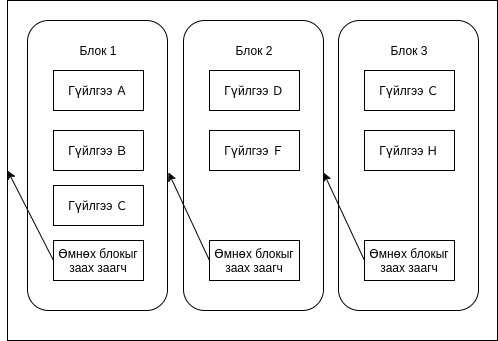
\includegraphics[scale=0.8]{src/images/blockchain-structure.jpg}
	\caption{Блокчейний өгөгдөлийн бүтэц}
\end{figure}

\textbf{Криптограф хэйш} функц нь оруулсан өгөгдлийн уртаас үл хамааран тогтсон урттай хэйш утгуудыг буцаадаг. Оролтын зөвхөн нэг тэмдэгт өөрчлөгдөхөд гаралтын хэйш утгууд нь эрс ялгаатай байна. Энэ шинж чанарыг ашиглан, гүйлгээний өгөгдөл болон бусад бүх өгөгдлийн хувьд засвар ороогүй болохыг баталгаажуулах боломжийг олгодог.

\textbf{Ухаалаг гэрээ} гэдэг нь дундын зуучлагч буюу хуульч, нотариатгүйгээр хоёр этгээд гэрээ байгуулсныг баталсан компьютерийн код бөгөөд тухайн гэрээний нөхцөл, үүрэг, хариуцлагыг багтаасан байна. Анх этереум нь ухаалаг гэрээг оруулсан блокчэйн гэдгийг гаргаж, түүний дараагаар олон тооны блокчэйнд ухаалаг гэрээг оруулж ирсэн. Ухаалаг гэрээ нь зөвхөн нөхцөл, үүргийг заахаас гадна автоматаар биелэх боломжтой байдаг.

\section{Блокчэйн зарим хэрэглээ}
Олон улсын хэмжээнд стартап компаниуд блокчэйн технологийг
ашигласан шинэ системийг эрүүл мэнд, даатгал, татвар зэрэг олон салбарт санал болгож байна.

Жишээлбэл, эрүүл мэндийн салбарт блокчэйн рүү иргэний эрүүл
мэндийн болон эмчилгээний түүхийг оруулдаг болгох систем юм. Энэ
тохиолдолд эмчлэгч эмч тухайн иргэний мэдээллийг харах судалгаа, шинжилгээний зорилгоор авч ашиглахаар бол системд хүсэлт гаргахад зөвхөн тухайн иргэний зөвшөөрлөөр системээс мэдээлэл нь харагдана. Хүний эрүүл мэндийн мэдээлэл блокчэйнд хадгалагдсанаар тухайн хүн дэлхийн аль ч улс оронд эмчилгээнд хамрагдахад асуудалгүй болж байгаа юм. Мөн блокчэйнд хүн өөрийн итгэмжлэгдсэн төлөөллийг нэмж өгөх боломжтой бөгөөд тухайн хүн өөрөө блокчэйнээс мэдээллээ гаргаж өгөх боломжгүй нөхцөлд ашиглагдах юм. Хэрэв блокчэйн ашиглагдаж эхэлбэл зайнаас эмчлэх, эмчилгээний зөвлөгөө өгөх зэрэг шинэ төрлийн үйлчилгээнүүд хүчээ авах юм.

\textbf{Нэгдсэн Үндэстний Байгууллага} 2017 онд блокчэйн технологи
ашигласан олон төрлийн санал, санаачлагыг хэрэгжүүлснээс үүний нэг болох тусламж түгээлтийн бүртгэлийн систем амжилттай хэрэгжсэн байна. НҮБ-аас гаргасан судалгаагаар, нийт тусламжийн 30 орчим хувь нь очих ёстой хүлээн авагчдаа хүрдэггүй гэж гарсан байна. 2017 оны тавдугаар сараас НҮБ-ын Дэлхийн хүнсний хөтөлбөрт хэрэгжсэн хүрээнд Сирийн дүрвэгчдэд үзүүлж байгаа тусламжийг этереум блокчэйн ашиглаж түгээжээ. Тодруулбал,
Иордан улсын дүрвэгчдийн хуаранд байрлаж байгаа Сири улсын 10500
дүрвэгчид хүнсний бүтээгдэхүүн (1.4 сая ам.доллар) түгээхэд криптовалютад суурилсан ваучер тарааж, уг ваучераа ашиглан хуаранд байрлах дэлгүүрээс хүнсний бүтээгдэхүүн авах боломжийг хангажээ. НҮБ-аас уг төслийг өмнөх тусламжтай харьцуулахад маш амжилттай хэрэгжсэн гэж үзэж байгаа бөгөөд 2018 оны хоёрдугаар улиралд тусламжинд хамрагдах хүний тоог 500,000-д хүргэхээр төлөвлөж байна гэж мэдээлж байна.

НҮБ-аас хамгийн сүүлд эхлүүлсэн нэг ажил нь хүүхдийг блокчэйнд
бүртгэлжүүлэх систем юм. Хуурамч бичиг баримт үйлдэн хүүхэд хил
дамнуулахыг зогсооход хамгийн ээдрээтэй зүйл нь жинхэнэ юм шиг
бүрдүүлсэн хуурамч бичиг баримтыг таних ажил байдаг. Хүний наймаа ихээр явагддаг бүс нутагт хүүхдүүдийг шат дараатайгаар албан ёсны бүртгэлтэй болгож, түүнийг нь НҮБ-ын блокчэйн системд хадгална. Энэ төрлийн гэмт хэрэг хамгийн их явагддаг Молдав улсад хэрэгжүүлж эхэлсэн ажээ. НҮБ-ийн судалгаагаар 5-аас доош насны хүүхэд бүртгэлжээгүй байх тохиолдол зарим
бүс нутагт их байдаг байна.

\textbf{Швейцарийн Зуг (ZUG)} хот нь крипто хот болохоор ажиллаж
байгаа бөгөөд ийм уриа гаргасан бусад хот болох Сан-Франциско, Лондон, Токио, Сингапур, Нью-Иорк, Амстердамаас ялгагдах зүйл нь санхүү болон технологийн гарааны бизнесээ эхэлж буй компаниудад хууль эрх зүйн орчин нь маш тааламжтай юм. Зуг хотын удирдлага крипто хөндий байгуулж, иргэдээ блокчэйнд бүртгэж эхэлсэн ба 2017 оны арваннэгдүгээр сараас иргэддээ зориулж цахим ID авах вебийн үйлчилгээг нээсэн нь этереум
блокчэйнд суурилсан ба хэрэглэгч хаанаас ч өөрийн мэдээллийг оруулан цахим ID-гаа авах боломжтой бөгөөд хотын зүгээс уг мэдээллийг зөвхөн шалгаж баталгаажуулах эрхтэй. Энэхүү цахим ID-гаа ашиглаад иргэд зөвхөн хотын үйлчилгээг (хэрэглээний төлбөр, түрээсийн төлбөр) авахаар хязгаарлагдахгүй ба 2018 оны хавар сонгуулийн санал өгөхөд (e-vote) ашиглахаар бэлдэж байна.